\chapter[Gaia cluster membership]{Open cluster membership in the \Gaia~era}
\label{chap:membership}

\section*{abstract}
    In this chapter we present cluster membership lists for the four open clusters in the nominal \Kepler~field of view. We used a Gaussian Mixture Model (GMM) machine-learning algorithm to determine cluster membership using astrometric (position and proper motion) data from the \Gaia~space telescope. We produced a cross-matched database for the \Gaia~and \Kepler~stars in the cluster fields of view. Our cluster membership list contains 
\newpage
\section{Cluster membership}

NGC 6791
One of the most studied open clusters


Previous cluster membership of NGC\,6791 \& NGC\,6819.
Historical studies

\section{The {\em Gaia} Mission}
The \Gaia~space telescope is a European Space Agency (ESA) mission launched in 2013 into a Lissajous-type orbit around the Lagrange-2 (L2) point, 1.5\,Mkm from Earth, in the anti-Solar direction. It was primarily designed to produce a three-dimensional astrometric map of the Milky Way. The full science goals of the mission were; (1) to map the positions of approximately 1 billion stars in the Milky Way and Local Group (to a precision of 24\,$\mu$as at 15\,mag and 200\,$\mu$as at 20\,mag), (2) to measure the proper motion velocities of these stars, (3) to produce a 3D structural map of the Milky Way, (4) to provide spectral and photometric measurements for these stars, and (5) to provide radial velocities for the 150 million brightest stars.

% \newpage

Figure \ref{fig:Gaia_structure} shows a schematic diagram of the \Gaia~spacecraft modules; the payload module containing the single, integrated science instrument, the mechanical service module and the electrical service module. The service modules are combined in this schematic to form the equipped service module, with the propulsion tanks, solar panel arrays and phase array antenna situated below it.

\begin{figure}[h]
    \centering
    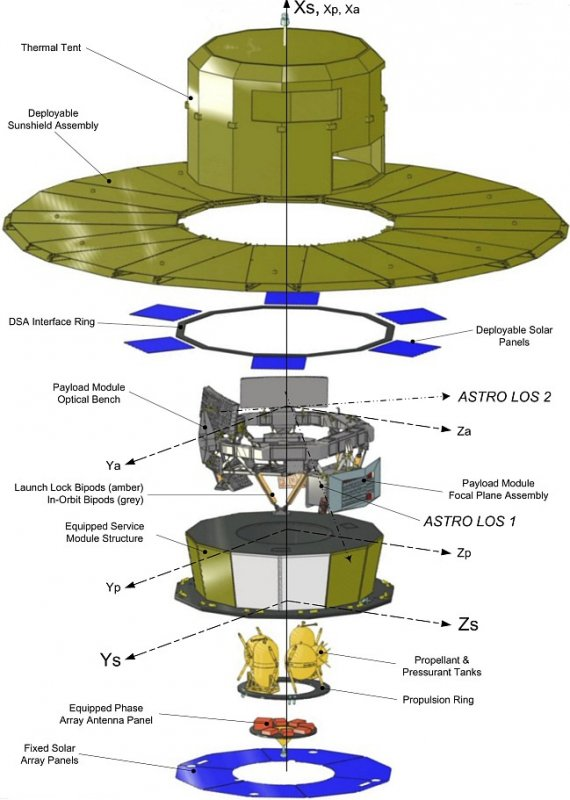
\includegraphics[width=0.6\linewidth]{Chapter4/gaia_schematic.jpg}
    \caption{Schematic diagram of the \Gaia~spacecraft. The electrical and mechanical service modules have been combined in this schematic into the `equipped service module structure', with the payload module displayed above.}
    \label{fig:Gaia_structure}
\end{figure}

The payload module contains the single, integrated instrument (Figure \ref{fig:gaia_instrument} (a)) responsible for delivering the astrometry, photometry and spectrometry data products. This instrument uses two identical telescopes with a shared focal plane, based on a three-mirror anastigmat design. A detailed schematic view of the optical path to the detector is shown in Figure \ref{fig:gaia_instrument} (b). The focal plane of the detector (Figure \ref{fig:gaia_focalplane}) has dimensions of 0.5\,m $\times$ 1.0\,m and consists of 106 CCDs that provide dedicated channels for each data product.

\begin{figure}[h]
    \centering
    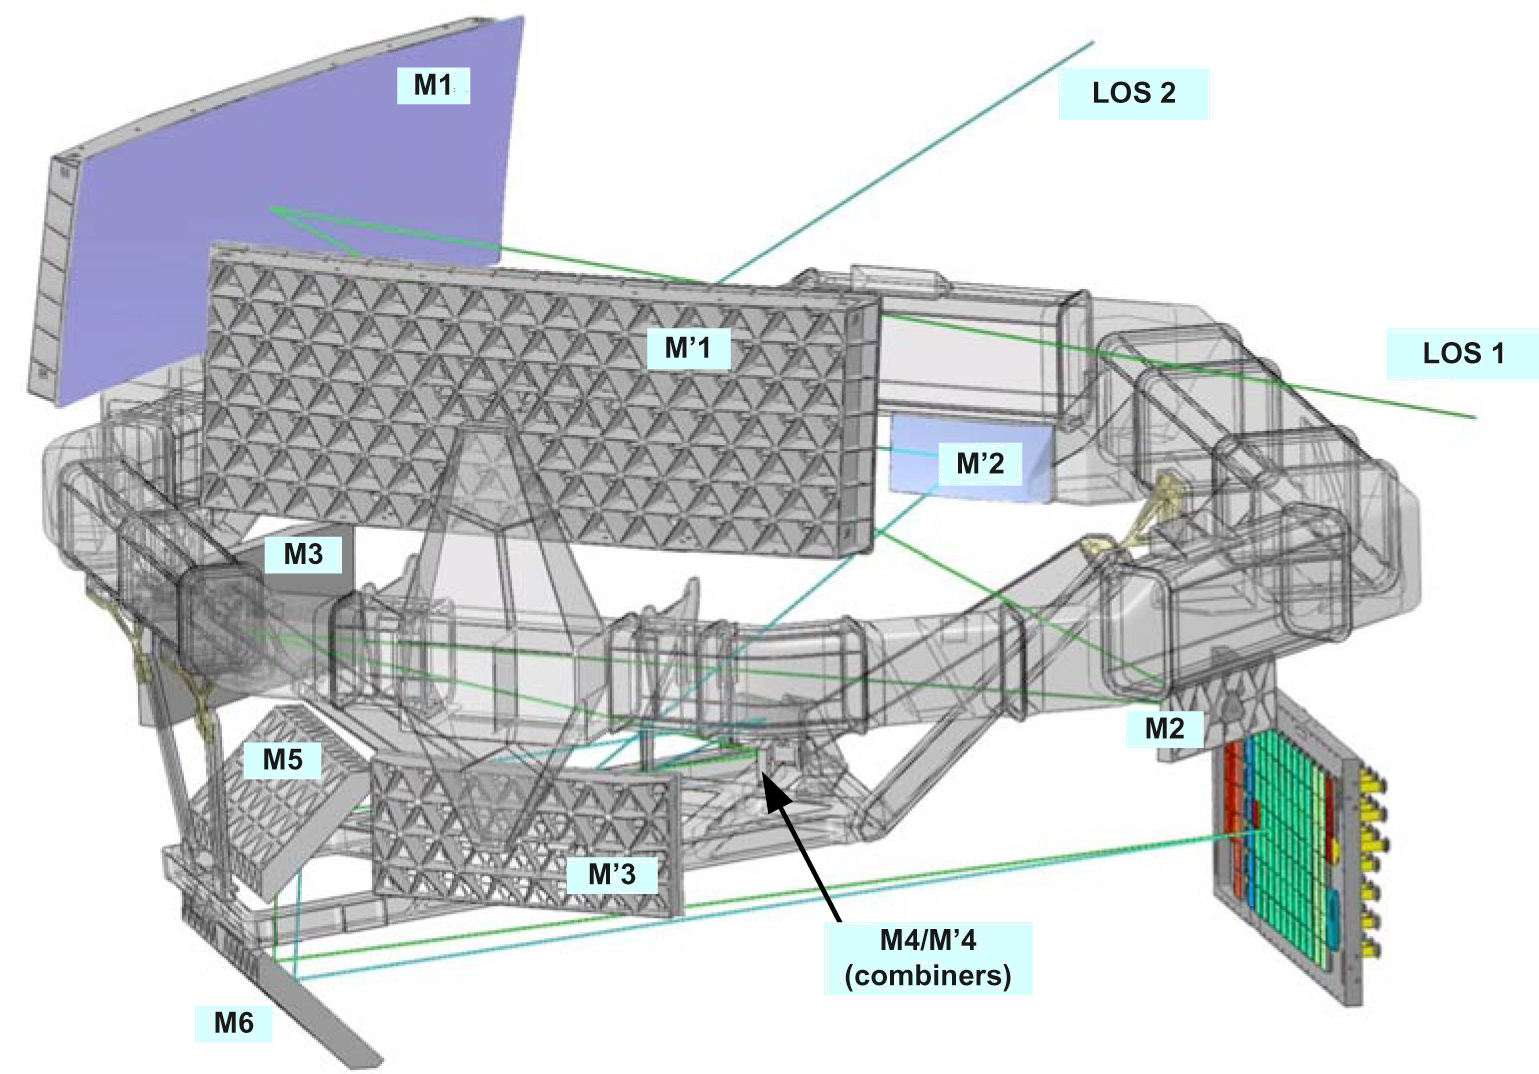
\includegraphics[width=0.8\linewidth]{Chapter4/gaia_optics.png}\\
    \vspace{25pt}
    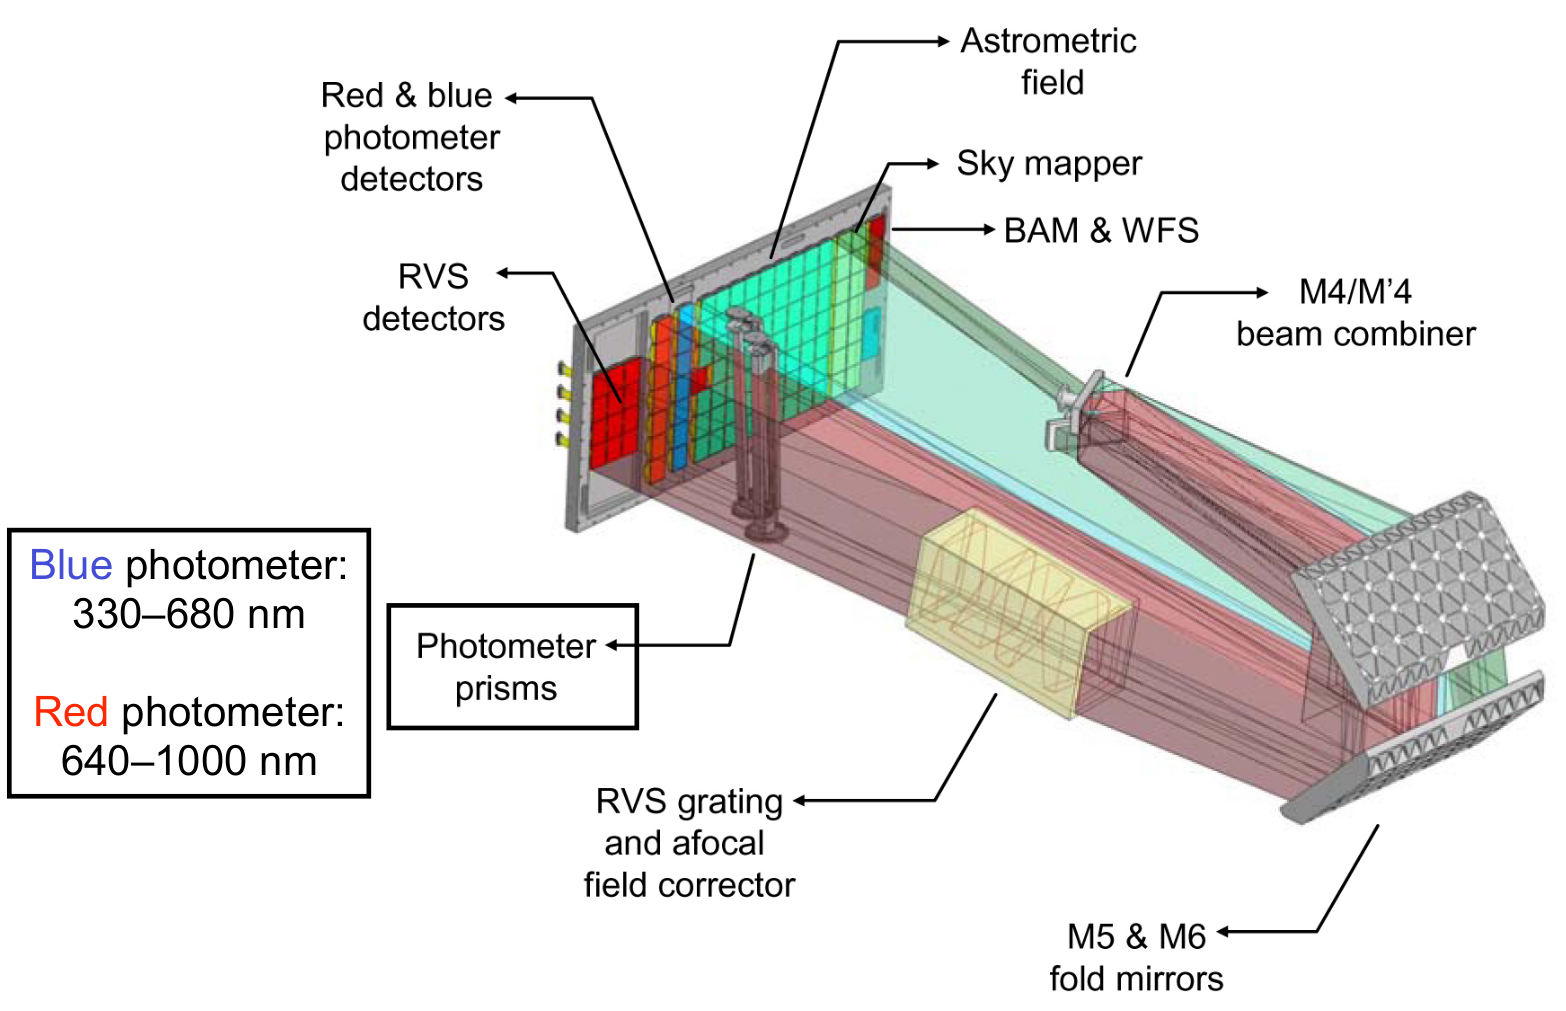
\includegraphics[width=0.8\linewidth]{Chapter4/gaia_foc.png}
    \caption{Schematic diagrams of (a) The \Gaia~optical instrument bench, and (b) The optical ray path from the M4/M'4 beam combiner to the focal plane containing the CCD detectors.}
    \label{fig:gaia_instrument}
\end{figure}

\begin{figure}[h]
    \centering
    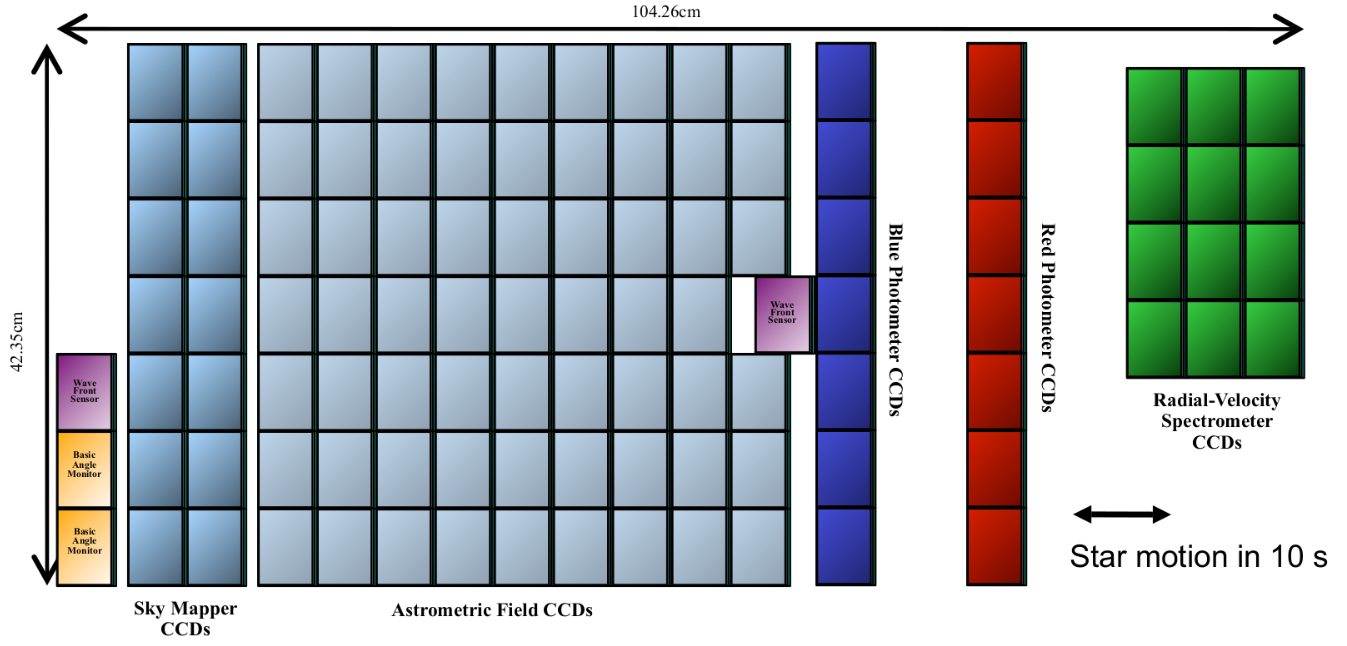
\includegraphics[width=0.9\linewidth]{Chapter4/gaia_detect_edit.png}
    \caption{Schematic diagram of the \Gaia~focal plane consisting of 106 CCDs, with the positions and dedicated instrument allocation of individual CCD modules annotated.}
    \label{fig:gaia_focalplane}
\end{figure}

\subsection{Astrometry}
The latest data release for the \Gaia~mission, Gaia DR2 (hereafter DR2), occurred in April 2018 \citep{gaia_collaboration_gaia_2018}. It contained five-parameter astrometric solutions ($\alpha$, $\delta$, $\mu_{\alpha}$, $\mu_{\delta}$, $\pi$) for 1.7\,billion stars, combined with photometric and spectrometric (G, G$_{BP}$, G$_{RP}$) magnitudes for 1.3\,billion stars. \citet{bailer-jones_estimating_2018} computed geometric distance estimates for all stars with a parallax in the DR2 release. We use both of these data products for the following analysis.

\section{Clustering methods}
We investigated a number of clustering algorithms to identify probable cluster members including Mean-Shift Clustering, Density-based Spatial Clustering of Applications with Noise (DBSCAN), and Expectation–Maximization (EM) clustering using Gaussian Mixture Models (GMM). We provide a description of how these algorithms function below, and discuss the benefits and limitations of each.

\subsection{Mean-Shift Clustering}

The mean-shift clustering algorithm locates local over-densities in N-dimensional data using a centroid-based, sliding window. The algorithm begins with a randomly-selected initialisation point at the centre of a radially-profiled kernel (e.g circular window in 2-D) in the parameter space. This kernel is iteratively shifted to higher density regions by calculating the mean of all enclosed points. The iterative shifting is concluded when the total number of points within the window no longer increases and convergence is achieved. 

This process is repeated with additional kernels until every data point in the parameter space is contained within a window, and thus assigned to a particular cluster. If multiple windows overlap, the window with the greatest density is preserved as the parent cluster, and the remaining windows eliminated.

The primary benefit of the mean-shift clustering algorithm is its ability to locate clusters without prior knowledge of the number of clusters present. This is offset by the need to tune the kernel radius hyper-parameter, a task that may be non-trivial. This process returns a binary classification of cluster membership and does not account for data points that may not be related to any particular cluster (ie noise).

\vspace{10pt}

\noindent{\bf Pros}: 
\begin{itemize}
    \item Automatically determines the number of clusters so no prior knowledge of clusters required.
\end{itemize} 

\noindent{\bf Cons}: 
\begin{itemize}
    \item Selection/tuning of the kernel radius hyper-parameter can be non-trivial.
    \item Binary classification to cluster only (member/non-member).
    \item Cannot account for noise in data set.
    \item Cannot account for clusters of varied density.

\end{itemize}

\subsection{Density-based Spatial Clustering of Applications with Noise (DB-SCAN)}

DB-SCAN is a classification algorithm designed to locate clusters of over-density within a given parameter space whilst accounting for the presence of non-members. 

The algorithm selects an arbitrary initialization point and calculates a distance metric for the given parameter space to all other data points. If there are a sufficient number of points, \texttt{min\_points}, within a given maximum separation, $\epsilon$, it classifies the point as belonging to a cluster, otherwise it is classified as noise. All data points within the $\epsilon$ distance vector of a cluster member are associated with the same cluster, and the classification repeated iteratively for each point, until all points within the $\epsilon$ neighborhood of the cluster have been added. This process is repeated for all unclassified data points, until all points have been assigned to a cluster or classified as noise.

DB-SCAN's main advantage over mean-shift clustering is the ability to account for noisy data where no cluster assignment is valid. It is also capable of locating clusters of arbitrary shapes and sizes. As with mean-shift clustering, DB-SCAN has difficulty accounting for varied cluster density, as the hyper-parameters will change from cluster to cluster. Tuning the hyper-parameters to account for normalised distances between parameter spaces can also be difficult, particularly with high-dimensional data.

\vspace{10pt}

\noindent{\bf Pros}: 
\begin{itemize}
    \item Automatically determines the number of clusters so no prior knowledge of clusters required.
    \item Can account for arbitrary cluster shapes and sizes.
    \item Can account for noisy data.
\end{itemize} 

\noindent{\bf Cons}: 
\begin{itemize}
    \item Selection/tuning of the distance, $\epsilon$, and minimum cluster members, \texttt{min\_points}, hyper-parameters can be non-trivial.
    \item Normalising dimensions, and thus calculating the $\epsilon$ hyper-parameter for high-dimensional data can be difficult.
    \item Binary classification to cluster only (member/non-member).
    \item Cannot account for clusters of varied density.
\end{itemize}

\subsection{Hierarchical DBSCAN (HDBSCAN)}

HDBSCAN is a variation of the traditional DBSCAN algorithm. It uses a hierarchical clustering algorithm to compensate for differences in cluster densities, allowing the identification of multiple clusters with different densities. 

hierarchical clustering algorithm, and then using a technique to extract a flat clustering based in the stability of clusters.

\subsection{Expectation-Maximization (EM) using Gaussian Mixture Modelling (GMM)}

Gaussian Mixture Models (GMMs) give us more flexibility than K-Means. With GMMs we assume that the data points are Gaussian distributed; this is a less restrictive assumption than saying they are circular by using the mean. That way, we have two parameters to describe the shape of the clusters: the mean and the standard deviation! Taking an example in two dimensions, this means that the clusters can take any kind of elliptical shape (since we have standard deviation in both the x and y directions). Thus, each Gaussian distribution is assigned to a single cluster.

In order to find the parameters of the Gaussian for each cluster (e.g the mean and standard deviation) we will use an optimization algorithm called Expectation–Maximization (EM).

We begin by selecting the number of clusters (like K-Means does) and randomly initializing the Gaussian distribution parameters for each cluster.
Given these Gaussian distributions for each cluster, compute the probability that each data point belongs to a particular cluster. The closer a point is to the Gaussian’s center, the more likely it belongs to that cluster. This should make intuitive sense since with a Gaussian distribution we are assuming that most of the data lies closer to the center of the cluster.
Based on these probabilities, we compute a new set of parameters for the Gaussian distributions such that we maximize the probabilities of data points within the clusters. We compute these new parameters using a weighted sum of the data point positions, where the weights are the probabilities of the data point belonging in that particular cluster.
Steps 2 and 3 are repeated iteratively until convergence, where the distributions don’t change much from iteration to iteration.There are really 2 key advantages to using GMMs. Firstly GMMs are a lot more flexible in terms of cluster covariance than K-Means; due to the standard deviation parameter, the clusters can take on any ellipse shape, rather than being restricted to circles.Secondly, since GMMs use probabilities, they can have multiple clusters per data point. So if a data point is in the middle of two overlapping clusters, we can simply define its class by saying it belongs X-percent to class 1 and Y-percent to class 2. I.e GMMs support mixed membership.


%\subsection{More realistic modelling}

\section{Methodology}

We used Gaussian Mixture Modelling (GMM) to calculate the posterior probability of membership for all stars within pre-determined radii of the four open clusters in the nominal \Kepler~field of view. We selected these radii to be approximately 2.5 times the literature reported radius for each cluster to ensure no potential cluster members were missed. Table \ref{tab:cluster_selection} presents the positions and radial distance cuts we used for each cluster. 

\vspace{3pt}

\begin{table}[h]
    \centering
    \setlength\tabcolsep{10pt}
    \begin{tabular}{ccccc}
        \hline
        Cluster     & RA        & Dec       & Radius    & Radial distance cut \\
                    &           &           & (arc mins)& (arc mins) \\
        \hline
        \hline
        NGC 6791    & 290.2208  & 37.771    & 23.0\footnote[2]{$r_t$ - Tidal radius \citep{platais_new_2011}} & 60.0\\
        NGC 6819    & 295.325   & 40.1867   & 15.0\footnote[2]{\citet{yang_wiyn_2013}} & 48.0\\
        NGC 6811    & 294.3208  & 46.3883   & 7.0               & 17.5\\
        NGC 6866    & 300.9792  & 44.1583   & 13.0              & 32.5\\
        \hline
    \end{tabular}
    \caption{Properties of open clusters in the \Kepler~FoV and the radial distance cut used for each cluster for cross-matching the \Gaia~and \Kepler~catalogs.}
    \label{tab:cluster_selection}
\end{table}

Data selected to try to ensure as close to complete membership as possible. Download \Gaia~DR2 data for all stars within the cutoff radius of the cluster centres. Due to distance of NGC 6819 \& 6791 we do not make a magnitude cut of this point despite the significant decrease in astrometric quality for stars fainter than G = 20 mag. Only a small fraction have RVs, with almost none of the cluster members from NGC 6791 having such values, so not used. Similarly, parallax values for these clusters are very small (distances are ~2 \& ~4 kpc respectively) meaning there is a very large uncertainty on their measurements. Due to this we did not use the parallax in the clustering analysis (See \cref{sect:cuts})

As reported by Lindegren et al. (2018) and confirmed
by several other works (Riess et al. 2018; Stassun \&
Torres 2018; Zinn et al. 2018), there is a zero-point offset
in the Gaia DR2 parallaxes that needs to be considered.
While this zero-point itself is a function of position and
magnitude, for the remainder of this paper we adopt the
global mean value of 29\,$\mu$as (in the sense that the Gaia
parallaxes are too small) reported by Lindegren et al.
(2018).

In order to derive reliable values for the cluster and
field parameters, we have used the subset of our initial
pool of stars that pass the quality cuts impossed by Zinn
et al. (2018) (which ensure a good astrometric solution)
and that are within 20 0 of the cluster center.(For similar samples in larger areas the field population is so dominant over the cluster that the latter becomes negligible and the method does not converge).

We used the position ($\alpha$ and $\delta$) and proper motion ($\mu_{\alpha}$ and $\mu_{\delta}\dot~cos\delta$) parameter space for all \Gaia~sources within the cutoff radius in our gaussian mixture model analysis. 
run sklearn gmm on (pmra,pmdec,ra,dec) with n components (6791 = 6, 6819 = 12). n$_{}$comp chosen based on initial runs where the minimum number of components needed to converge to cluster members is accepted. Iteratively repeat using Monte Carlo (gaussian function over ($pmra_err,pmdec_err,ra_err,dec_err$)) to sample the parameter space. Accept cluster if 50$\%$ of members from initial run included in one component of the current GMM convergence, otherwise reject.

Cluster:	6819 | 6791	
Position:	[295.325, 40.1867] | [290.2208, 37.771]
radius cut:	0.8	| 1.0
gmm tol:	1e-5       
gmm maxiter:	20000      
gmm cov:	full       
gmm weight:	dirichlet distribution

Include the images showing the probability distribution of highly-likely, likely, non-likely members and some which are ambiguous.

Describe choices made about membership and show results.

6791


6819

\section{Results}

\label{sect:cuts}

\begin{figure}
\centering
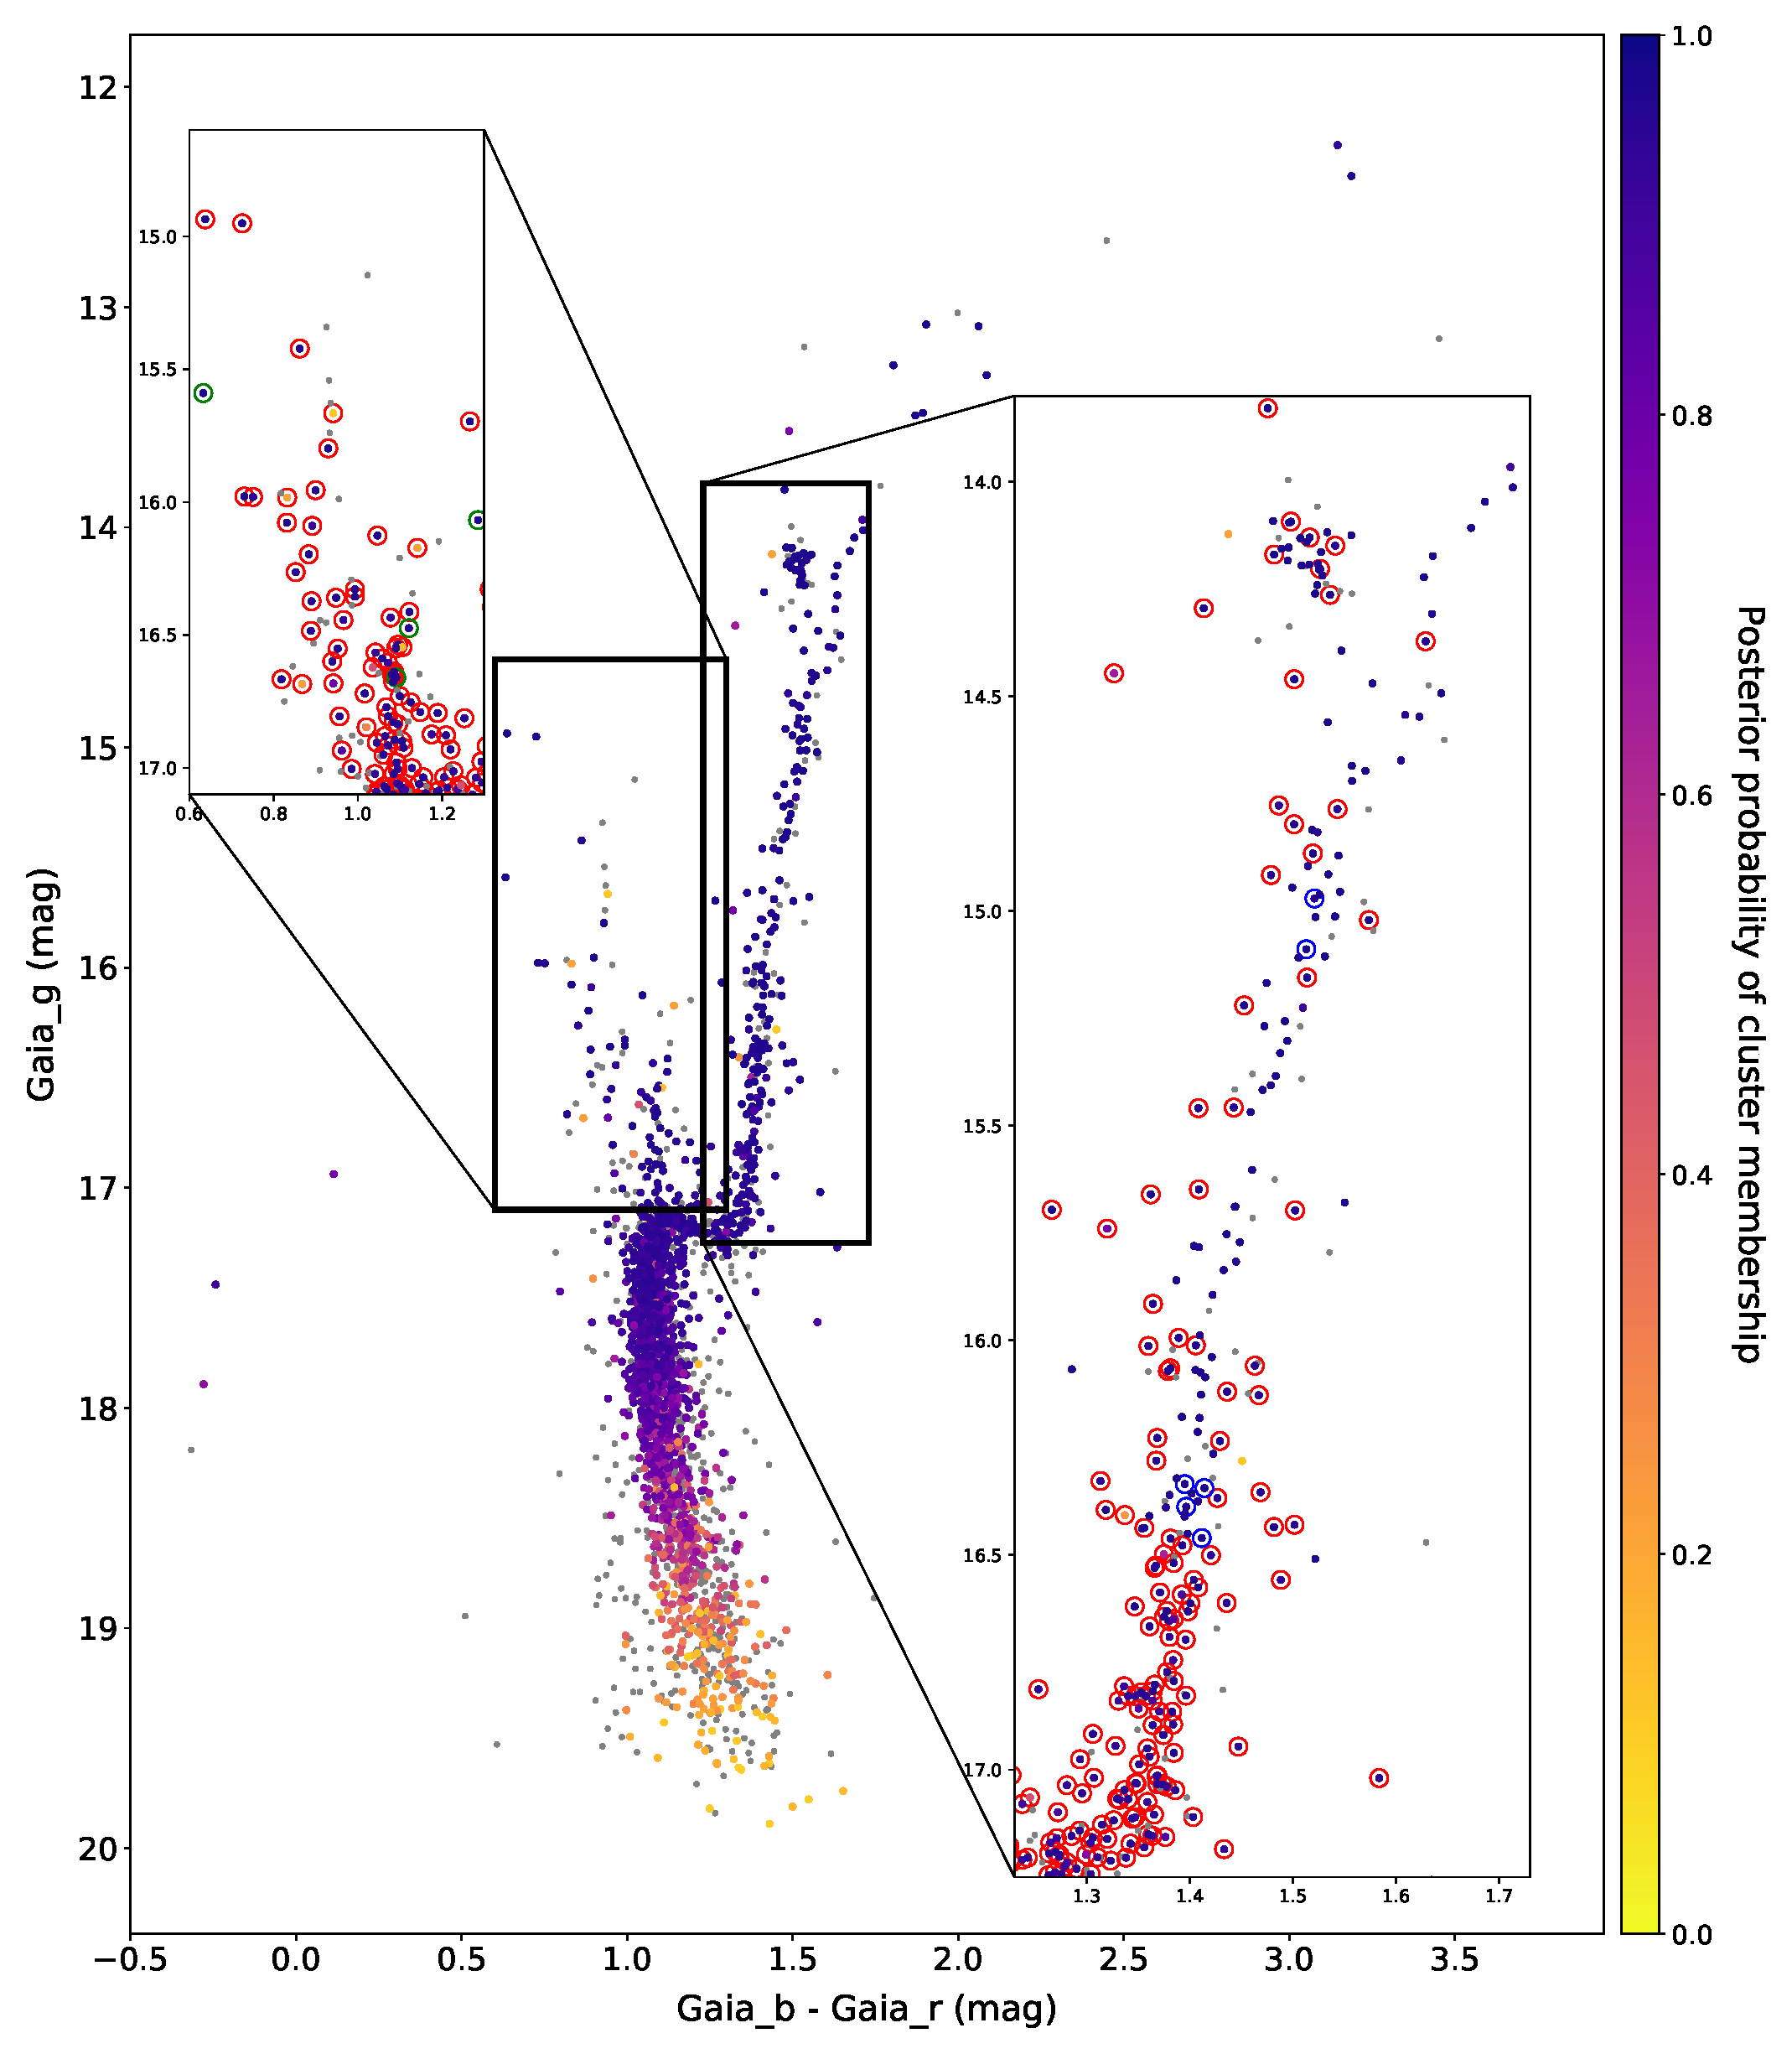
\includegraphics[width=\linewidth]{Chapter4/cmd_6791.eps}
\caption[NGC\,6791 CMD]{Colour magnitude diagram of NGC\,6791 based on \Gaia~$g$ and $b-r$ passband photometry, showing likely cluster members (gray) with those that fall inside the \Kepler~super stamps shaded by their posterior probability of membership. The red giant branch (right insert) and blue straggler stars (left insert) are highlighted. For these regions we have further highlighted the non-targeted super stamp stars (red circles, both), red giants observed for less than nine quarters (blue circles, right), and observed blue stragglers (green circles, left)}
\end{figure}

\begin{figure}
\centering
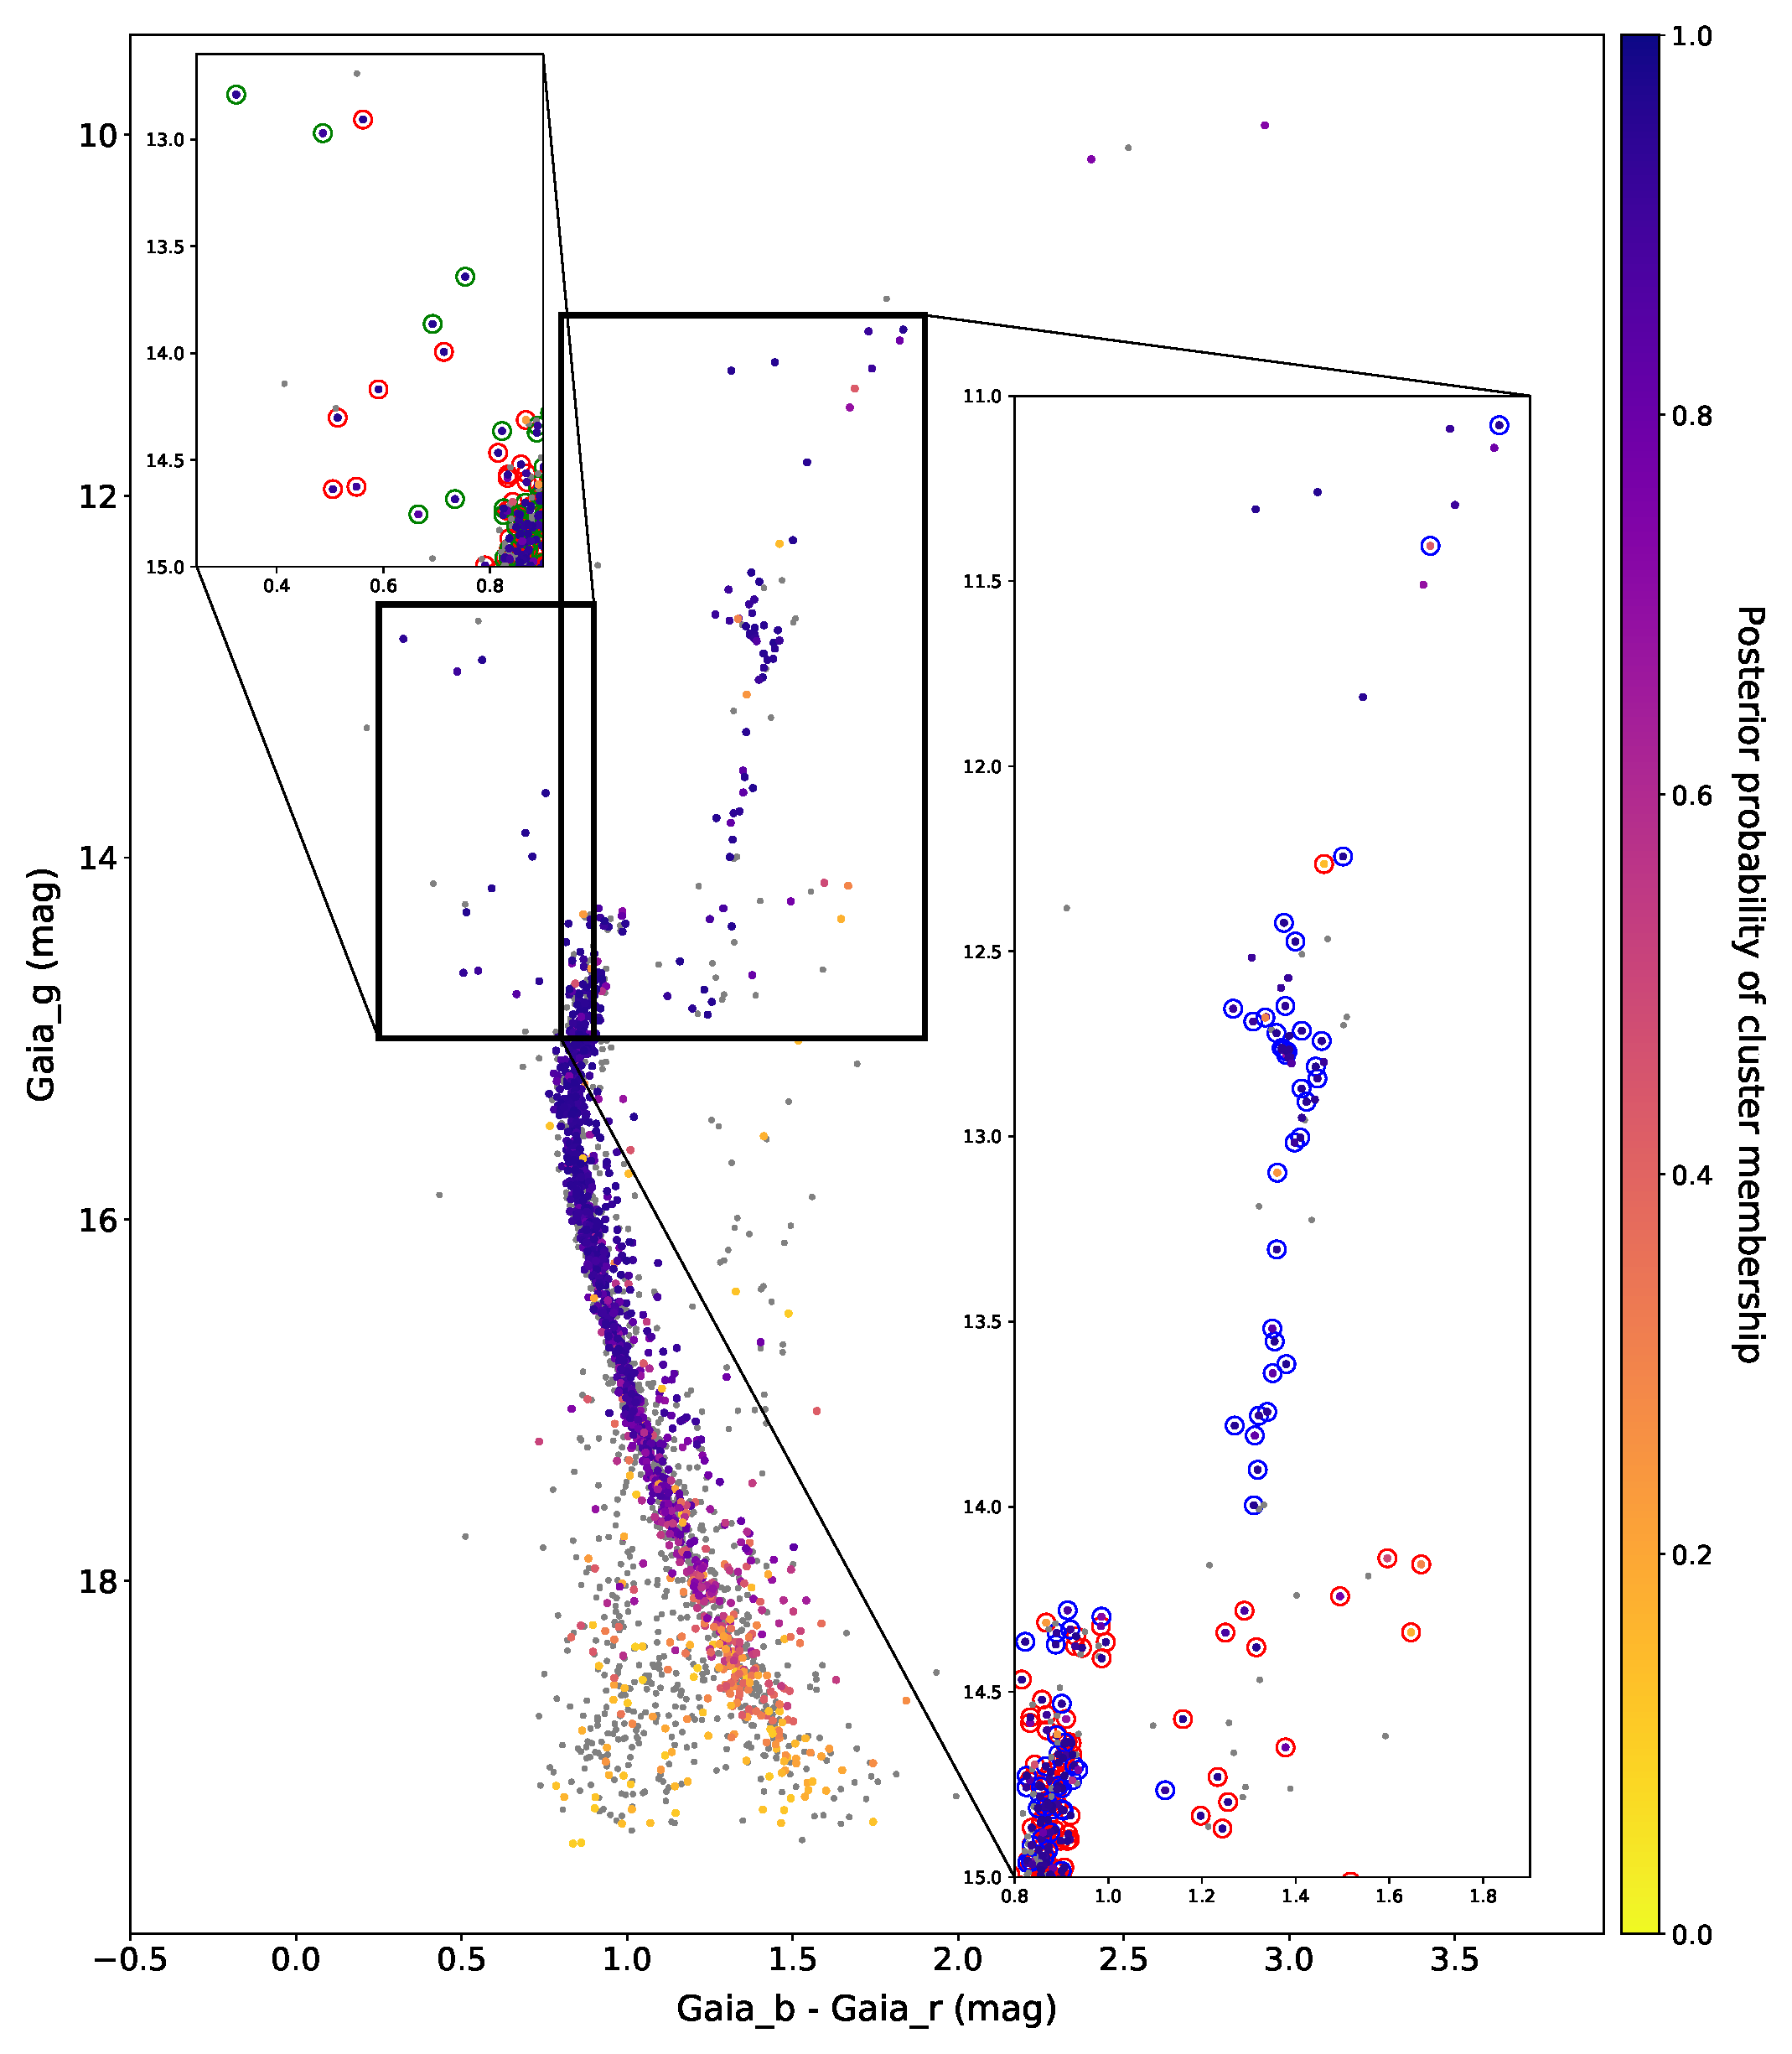
\includegraphics[width=\linewidth]{Chapter4/cmd_6819.eps}
\caption[NGC\,6819 CMD]{Colour magnitude diagram of NGC\,6819 based on \Gaia~$g$ and $b-r$ passband photometry, showing likely cluster members (gray) with those that fall inside the \Kepler~super stamps shaded by their posterior probability of membership. The red giant branch (right insert) and blue straggler stars (left insert) are highlighted. For these regions we have further highlighted the non-targeted super stamp stars (red circles, both), red giants observed for less than fifteen quarters (blue circles, right), and observed blue stragglers (green circles, left)}
\end{figure}

\subsection{Kepler-Gaia DR2 Cross-matching}

% To combine this astrometric analysis with the photometric (and thus asteroseismic) {\em Kepler} information we need to match the {\em Kepler} and {\em Gaia} identifiers.

\citet{berger_revised_2018} produced a \Gaia~cross-matched database for all \Kepler~targeted stars to allow for astrometric analysis of these stars, but excluded non-targeted cluster stars. We have now extracted light curves for many of these non-targeted stars within the centres of the open clusters in the nominal \Kepler~FoV from the \Kepler~superstamps (%\citet{Colman19}, 
Ch. \ref{chap:lightcurves}). These stars are now of particular interest in terms of cluster membership for conducting ensemble asteroseismic analyses, and require a cross-match between \Kepler~and \Gaia~identifiers.

% Before cross-matching the \Gaia~and \Kepler~catalogs, we converted the Gaia stellar positions ($\alpha$, $\delta$) from the J2015.5 reference frame to the J2000.0 reference frame used by the \Kepler~Input Catalog (KIC) \citep{brown_kepler_2011}. 
Before cross-matching the \Gaia~and \Kepler~catalogs, we corrected the Gaia stellar positions ($\alpha$, $\delta$) for proper motion to the J2000.0 epoch. We then restricted the cross-match to stars within a radius of each cluster centre matching the cluster radius selected for the cluster membership analysis (see Table \ref{tab:cluster_selection}). 

To begin the cross-match, we removed all KIC stars without a \Kepler~magnitude (Kp). For every \Gaia~star, we selected all matches within an initial 3 arcsecond radius. We further filtered the matches by imposing a magnitude cut based on the \Gaia~g-band photometry and \Kepler~magnitude to ensure ${|g-Kp| \leq 2}$, and selected the closest star as the best match. For any duplicate \Kepler~matches we selected the \Gaia~match with the smallest angular separation as the best match. We then removed this \Kepler~match from the possible matches, and iteratively repeated the cross-match until all stars were matched or no match was found. 

Finally, we removed all matches with angular separations greater than 1.5 arcseconds. We selected 1.5 arcseconds based on a 5\,$\sigma$ interval from a truncated Gaussian fit to the angular separation distribution. We assume any matches beyond this angular separation are likely to be spurious background or foreground contaminants as suggested by \citet{berger_revised_2018}. We present the number of stars included at each stage of the cross-match, for each cluster field of view, in Table \ref{tab:cluster_crossmatch}.

%Could not use APASS gri photometry to fill in Kepler data and generate predicted G mag as Berger due to cluster members typically being much fainter than the limiting cutoff mag for APASS.
\begin{table}[h]
    \centering
    \setlength\tabcolsep{10pt}
    \begin{tabular}{ccccc}
        \hline
        % Cluster     & RA        & Dec       & Radius    & Radial distance cut \\
        %             &           &           & (arc mins)& (arc mins) \\
        % \hline
        % \hline
        % NGC 6791    & 290.2208  & 37.771    & 23.0\footnote[2]{$r_t$ - Tidal radius \citep{platais_new_2011}} & 60.0\\
        % NGC 6819    & 295.325   & 40.1867   & 15.0\footnote[2]{\citet{yang_wiyn_2013}} & 48.0\\
        NGC 6811    & 294.3208  & 46.3883   & 7.0               & 17.5\\
        NGC 6866    & 300.9792  & 44.1583   & 13.0              & 32.5\\
        \hline
    \end{tabular}
    \caption{Number of stars present in the cross-matched database at each stage.}
    \label{tab:cluster_crossmatch}
\end{table}


NGC 6791  [125\,018 KIC stars and 153\,626 \Gaia~stars] to begin the cross-match.




% For stars with multiple matches that satisfied these criteria, we decided to keep those with the smallest angular separations. Of the 197,104 stars present in the KSPC, we identified Gaia DR2 source matches for 195,710. Stars with poorly determined parallaxes (σ π /π > 0.2), low effective temperatures based on our adopted values (T eff < 3000 K, see Section 2.2), extremely low log g (< 0.1 dex), and/or non-“AAA”-quality Two Micron All Sky Survey (2MASS) photometry were rejected from our sample.

% Additionally, we made astrometric cuts similar to those described in Appendix C of Lindegren et al. (2018) and Section 4.1 of Arenou et al. (2018). In particular, we used Equation (1) (unit weight error compared to a function of the G magnitude of the source that helps filter contamination from binaries and calibration problems) and Equation (3) (greater than eight groups of observations separated by at least 4 days) of Arenou et al. (2018) to remove stars with bad astrometric solutions. We did not use the astrometric excess noise values provided by Gaia DR2 to filter stars because they were less discriminating for stars with G < 15 due to the “degree of freedom bug” (see Appendix A and C of Lindegren et al. 2018). We did not use Equation (2) of Arenou et al. (2018), a cut ensuring that Gaia has clean photometry of the included sources, because we utilized separate 2MASS photometry in our analysis. As discussed in Lindegren et al. (2018), our imposed cuts removed many stars that appear in unphysical areas of radius-T eff parameter space, such as the “subdwarfs” between the stellar main sequence and the white dwarf branch. Excluding these stars reduced our final sample to 177,911 Kepler stars.

% Methodology:
% Position, pm and colour-photometry from Gaia - g, b, r => Conversion to Kepler (Kp) magnitudes

% Match on Kp (calculated) and measured -> remove any greater than 2mags
% Closest match

% Results:

Database of Kepler and Gaia ID's including the information from both databases. (Include table of ~20 examples [<= 1 page] with extended match online)